\section{Introduction}

In recent years, Machine Learning algorithms have received much attention due to their efficiency in solving otherwise difficult classification tasks.
Amongst others, there are applications in spam filtering \cite{ruan2010three, clark2003neural}, malware detection \cite{dahl2013large}, natural language processing \cite{collobert2008unified} and image classification \cite{simonyan2014very, he2016deep}.
In the latter domain, deep neural networks (DNNs) and especially convolutional neural networks (CNNs) have become very popular.
However, recent research has also shown that these ML algorithms are vulnerable to crafting malicious inputs, called \enquote{adversarial examples}.
These inputs are created by an attacker with the intention of tricking the machine learning system into misclassifying.
\citet{szegedy2013intriguing} were the first to explore this kind of evasion attack aimed at finding unnoticeable modifications to a valid input sample such that it is misclassified by the DNN but still looks the same to a human observer.

This year's InformatiCup challenge revolves around a related topic: The task is to generate images which do not look like traffic signs but are classified as such by a remote model with a high confidence (90\%).
Because image classification is used for self-driving cars which automatically detect and classify traffic signs, this issue is equally topical and relevant.
It is an essential goal to prevent self-driving cars from being mislead by these adversarial examples since this could potentially endanger human lives.
Considering a situation in which someone places a sticker on the back of a lorry which looks benign to humans but is classified as a yield sign by a car, the criticality of this topic becomes very clear.
This motivates exploring different kinds of attacks against ML algorithms in order to better understand the vulnerabilities, paving the way for setting up effective defenses.
Adversarial Examples themselves are an active research direction and though there exist a plethora of attacks, it's neither clearly established why adversarial examples exist nor how to effectively defend against them.

One of the most prominent projects for benchmarking defenses is the CleverHans project in which several state-of-the-art attacks are included \cite{papernot2016cleverhans}.
By leveraging these existing algorithms and creating custom extensions to them, this work contributes to a better understanding of how these adversarial examples can be generated and physically applied.
For example, perturbations are only valid for a single image in most cases, which has been taken from a certain angle.
In the situation of a self-driving car passing by an adversarial example, this would only trigger in a fraction of a second.
To cover a more realistic scenario, we implemented a modified attack which makes these adversarial examples robust against being seen from different angles.

On a more detailed level, the scenario of this challenge is similar to the \enquote{rubbish class examples} described by \citet{szegedy2015explaining}, which are images that a human would not assign any of the given classes.

An obstacle in the competition is the access to the remote model, which is only accessible via a web interface,
reporting the top five most-likely classes and their confidences for a given image.
This means that the architecture, the weights and the training hyperparameters are unknown, which are critical to most attacks that generate adversarial examples.
This impediment is overcome by \citet{papernot2017practical} which turn the limited access into a white box model.
Therefore, the challenge of this task lies in combining multiple insights of adversarial research and applying them in a real-world situation.

\begin{figure}
\vspace{4ex}
\centering
\begin{subfigure}{.19\linewidth}
  \centering
  
\includegraphics[width=0.7\linewidth]{imgs/octocat}
\end{subfigure}
\begin{subfigure}{.19\linewidth}
  \centering
  
\includegraphics[width=0.7\linewidth]{imgs/4}
\end{subfigure}
\begin{subfigure}{.19\linewidth}
  \centering
  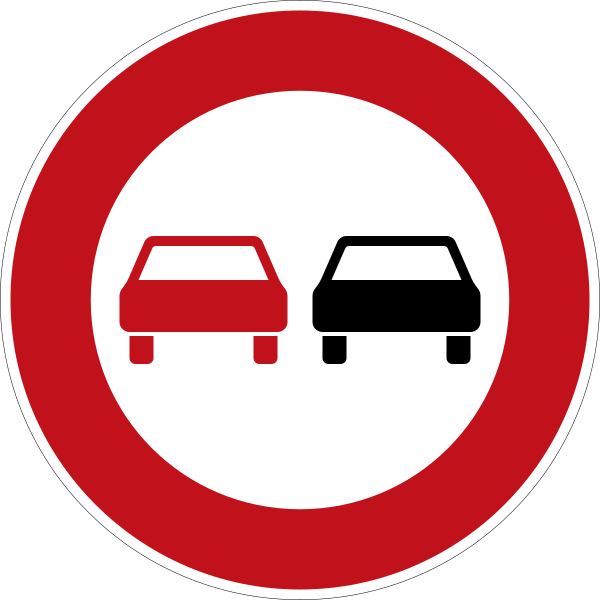
\includegraphics[width=0.7\linewidth]{imgs/4_real}
\end{subfigure}

\begin{subfigure}{.19\linewidth}
  \centering
  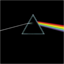
\includegraphics[width=0.7\linewidth]{imgs/darkside}
\end{subfigure}
\begin{subfigure}{.19\linewidth}
  \centering
  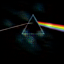
\includegraphics[width=0.7\linewidth]{imgs/7}
\end{subfigure}
\begin{subfigure}{.19\linewidth}
  \centering
  
\includegraphics[width=0.7\linewidth]{imgs/7_real}
\end{subfigure}

\begin{subfigure}{.19\linewidth}
  \centering
  
\includegraphics[width=0.7\linewidth]{imgs/gi}
\end{subfigure}
\begin{subfigure}{.19\linewidth}
  \centering
  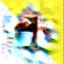
\includegraphics[width=0.7\linewidth]{imgs/10}
\end{subfigure}
\begin{subfigure}{.19\linewidth}
  \centering
  
\includegraphics[width=0.7\linewidth]{imgs/10_real}
\end{subfigure}
\caption{Excerpt from our results: Each row contains from left to right an input image, an adversarial example and a typical target class image.}
\label{fig:eyecatcher}
\end{figure}

An excerpt from our results is shown in Figure \ref{fig:eyecatcher}. 
Each row contains the source image on the left, the result from the attack in the center and an image of the falsely classified label by the remote model on the right.
A thorough explanation of how these example have been created as well as a discussion about the result quality can be read in the remainder of this paper, which is organized as follows:

At the beginning, we provide the background information required to understand our approach in Section~\ref{sec:background} and describe the prevalent threat model in Section~\ref{sec:threatmodel}.
After that, the theoretical approach as well as the software development and testing strategy are explained in Section~\ref{sec:methodology}.
Our implementation's architecture is presented in Section~\ref{sec:arch}.
Section~\ref{sec:results} shows our submitted images with a brief explanation of our results which are thereafter evaluated in Section~\ref{sec:evaluation}.
At the end, we present possible future extensions in Section~\ref{sec:extensibility}, discuss the general quality of our solution in Section~\ref{sec:discussion} and conclude our results in Section~\ref{sec:conclusion}.